\documentclass[10pt]{article}
\usepackage[breaklinks=true]{hyperref}
\usepackage[margin=0.75in]{geometry}

\usepackage{color}
\usepackage{graphicx}
\definecolor{pblue}{rgb}{0.13,0.13,1}
\definecolor{pgreen}{rgb}{0,0.5,0}
\definecolor{pred}{rgb}{0.9,0,0}
\definecolor{pgrey}{rgb}{0.46,0.45,0.48}

\usepackage{listings}
\lstset{language=bash,
  showspaces=false,
  showtabs=false,
  breaklines=true,
  showstringspaces=false,
  tabsize=2,
  breakatwhitespace=true,
  commentstyle=\color{pgreen},
  keywordstyle=\color{pblue},
  stringstyle=\color{pred},
  numbers=left,
  stepnumber=1,
  basicstyle=\small\ttfamily,
  frame=single,
  moredelim=[il][\textcolor{pgrey}]{$$},
  moredelim=[is][\textcolor{pgrey}]{\%\%}{\%\%}
}

\title{\textbf{Week 09} \\
\Large How Does The Internet Work? Python, cURL and a REST API}
\author{
	Melvyn Ian Drag
}
\date{\today}


\begin{document}
\maketitle

\begin{abstract}
This Lecture is preamble to the next one in which we will set up an apache webserver. We'll take a peek at Python, revisit cURL, and make some web requests.
\end{abstract}


\section{Exam Make Up}
Folks who missed the exam last week can come early and work until 7:15 to get it done. Lecture starts promptly at 7:15.

\section{Python Webserver}
\subsection{What is Python?}
Python is a scripting language kind of like bash or javascript or perl - but different. It's the favorite language of legions of programmers. Python is used everywhere from scientific computing - I used it to solve PDEs in grad school - to game development, to system administration, to excel spreadsheet modifying, to a million other use cases. Today we're going to look at Python as a language for making websites and serving webpages.

\subsection{What is a webserver?}
As we discussed before, when type a website into a browser ( like Chrome or Firefox, or the like ) and hit \textit{ENTER}, you ask a webserver for some information. The webserver responds with the information you requested and you see a webpage. This type of transaction is called a \textbf{GET} request when performed over the \textbf{Hyper Text Transmission Protocol (HTTP)} or the related \textbf{HTTPS}, which is the secure flavor of HTTP. We'll discuss what we mean by `secure' in a few weeks. 

Another thing you do when talking to a website is give some data to a webserver. This happens when you type your First Name, Last Name, User Name, phone number, password, etc. into a form on a website and click \textit{Submit}. When you click the button, the browser sends a \textbf{POST} request to the webserver that is listening to you from some other corner of the earth. 

In the case of either a GET or POST request, the request goes to a webserver, which is a computer far far away from you that has some code running on it that will respond to your GETs and your POSTs. That code is very often written in Java. It is frequently written in Python. Many write that code in Ruby. Many others use Scala to write the web server code. Recently, people started using Javascript to write the server code. 

In this class we will write the server code in Python.

\subsection{Install Python 3.}

Install it with 

\begin{lstlisting}
user@machine$ sudo apt install python3-dev
\end{lstlisting}

\subsection{Don't install Python 2}
Python 2 is being deprecated next year. The Python language maintainers have been telling the Python community to move to Python3 for about 10 years now. If you are new to Python, use Python 3. If you are old to Python, hurry up and port your code to Python 3!

\subsection{Simple Python Webserver}
Okay, so now that you have Python installed, we can set up a simple web server and begin to make some HTTP GET and SET requests!

Here is the code:
\lstinputlisting[language=Python]{Server.py}

This code is available in the class repository under the name \textit{Server.py}. From just this simple little example, we can learn alot about how the internet works. As we survey the example, we can issue some curl requests and verify that they work.

We can run this code from the command line with:

\begin{lstlisting}
user@machine$ python3 Server.py
Starting httpd server on localhost:8000
\end{lstlisting}

So we see that our little baby website is running on "localhost" at port 8000. Standard HTTP applications run on port 80, but for this demo app we are running on port 8000. Just for reference - HTTPS applications run ( by default ) on port 443. And ssh is over port 22. And postgresql is on port 5432. So now you know 4 special ports!

A summary of what we know about ports so far:
\begin{itemize}
\item port 22 - ssh
\item port 80 - HTTP
\item port 443 - HTTPS
\item port 5432 - PostgreSQL
\end{itemize}

In the webdevelopment world, we make \textbf{GET} and \textbf{POST} requests to webservers that have IP Addresses. But we rarely refer to them by their ip address - typically we use a domain name like `www.google.com' instead of a number address. We are doing the same thing here - we name our local webserver "localhost" instead of referring to it by its numeric name - 127.0.0.1 

\subsection{A quick look at the code}

Note that there are methods for handling \textbf{POST} and \textbf{GET} requests. This is characteristic of code running on a webserver. The code will have methods for handling different types of HTTP requests. You'll also see a few lines of code for setting up an HTTP server to run on `localhost:8000'. Theres a line that does something or other with ``headers", and we'll look into those in a minute. And there's a function that does something with html. If you've never seen HTML before, that's what it looks like. It's a markup language. If you don't know what HTML is, you can learn it in just a few minutes, it's pretty simple. It structures a document between some brackets. HTML always looks something like this:

\begin{lstlisting}[language=HTML]
<html>
<body>
	<h1> This is a title </h1>
	<h2> This is a subtitle </h2>
	<div> This is a paragraph about something </div>
</body>
</html>
\end{lstlisting}

\subsection{Verify Website Works With A Browser}
To verify that our website is running, open a broswer window (chrome, firefox, etc) and type "localhost:8000". You should get a response like this:

\begin{figure}[h]
  \centering
    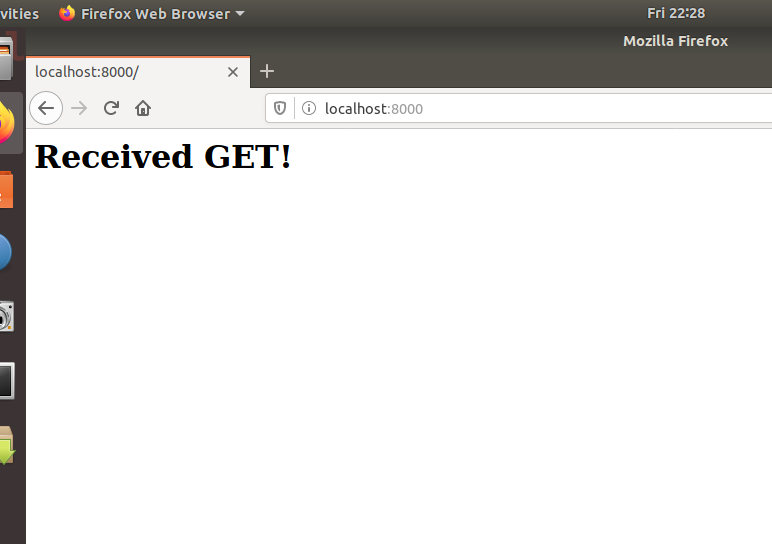
\includegraphics[width=0.5\textwidth]{GET.png}
  \caption{GET request in browser to localhost:8000}
\end{figure}

So we know our website "localhost:8000" is running.

And as I mentioned before, ``localhost" is an alias for ``127.0.0.1", which we can readily verify by going to ``127.0.0.1:8000" while our little application is running.

\begin{figure}[h]
  \centering
    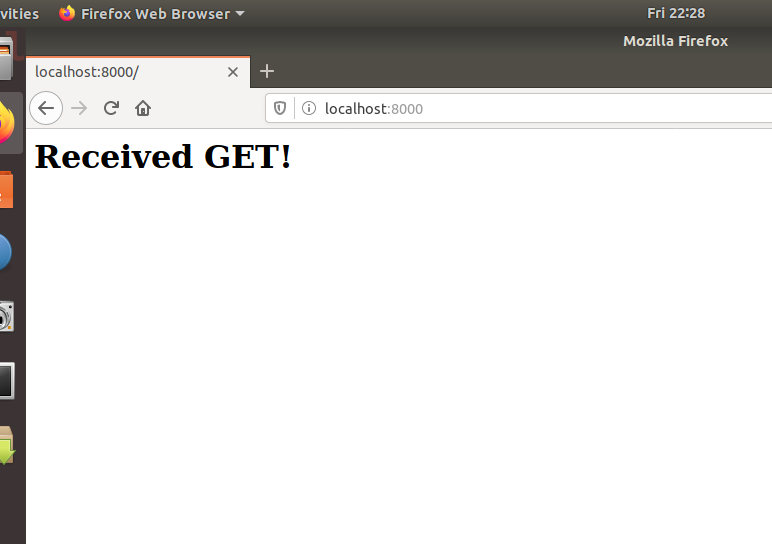
\includegraphics[width=0.5\textwidth]{GET.png}
  \caption{GET request in browser to 127.0.0.1:8000 }
\end{figure}

One more thing of interest - in case you've never seen this happen before - is you can see the Server code handling reqeusts on the server side. Go back to the terminal window where the webserver is running and you'll see it logging output after handling every request.

\begin{figure}[h]
  \centering
    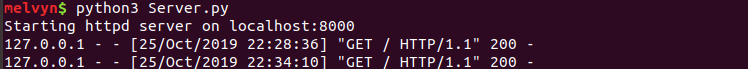
\includegraphics[width=0.5\textwidth]{GET_ServerSide.png}
  \caption{See the webserver handling the GET request traffic. }
\end{figure}

You may be frustrated because something doesn't match up with your expectations here. We see a website in a browser, but how come we don't type ``www.something.com"??? What is this ``localhost" nonsense? What do you mean it's running on port 8000??? I thought you said something or other about port 80 being for http??? All this understanding will come with time. For now we just need to know that websites handle GET and POST requests ( and other types of requests too ). And we've seen a little bit of code that features a get and post handler, and we've verified that ( the GET at least ) works as expected.

Now enough fooling around! Let's use cURL to test out our little website.

\section{Two Exercises}
\begin{center}
\textbf{ \#1 : Change port 8000 in the code to port 80 and try to rerun.}
\end{center}

Some ports are specified for a specific purpose by the os and may require special permissions to use. For example, port 80 requires root access to use. You can try to change the port 8000 in the sample code to port 80 and you will see a permission denied error unless you use sudo.

\begin{figure}[h]
  \centering
    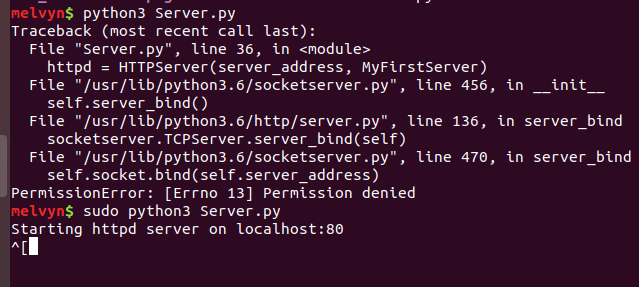
\includegraphics[width=0.5\textwidth]{needRootFor80.png}
  \caption{Need Root Access for Port 80}
\end{figure}


\begin{center}
\textbf{\#2 : Change `localhost' in the code to `127.0.0.1'. Note that is runs as expected - localhost and 127.0.0.1 are the same thing.}
\end{center}

If ip addresses interest you, like, why was `127.0.0.1' selected as `'localhost'? Are there other ip addresses that were designated as local ip addresses? Then you should learn more about computer networking! I admit that I'm very interested in the subject, but haven't studied it enough due to other responsibities and ambitions.

\section{cURL}
cURL is a Linux tool that has been around for about 20 years. It's used for making requests. It can be thought of as a command line browser, in some sense. The things you usually do  in a browser, like typing an address into a search bar, entering data into a form on a web page, clicking a button - these things can be done on the command line with cURL ( mostly ).

\subsection{Exercise \#1}
Open another terminal window in addition to the one running your Python webserver. Then enter these commands:

\begin{lstlisting}
user@machine$ curl localhost:8000
# returns some html from the website
user@machine$ curl -X GET localhost:8000
# returns the same thing, because the default curl action is GET
user@machine$ curl -X POST -d"myname=melvyn" localhost:8000
# returns the POST response, along with the data you passed in
user@machine$ curl -X POST --verbose -d"myname=melvyn" localhost:8000
# returns the same thing, but this time with lots of extra information!
# this time you can see what you sent over via the POST in detail
# along with a detailed response from the server
# The lines with a > are what you sent.
# The lines with a < are what came back.
user@machine$ curl -X POST --verbose -d"myname=melvyn&mylastname=drag" localhost:8000
# Try sending more and more data values by separating them with an ampersand.
\end{lstlisting}


The `-X' flag is used for specifying the HTTP verb associated with your request. As you've seen, the webserver will contain code for handling different types of requests.

The `-d' flag is used for passing data. Typically we associate the `-d' flag with POST requests and not GET requests.

\subsection{Headers}
As with most other data transmission protocols, file formats, etc. - most computer data formats - there is a header, followed by a body. What are HTTP headers?


\subsection{Congratulations!}
You may have just run your first webserver! If this wasn't your first webserver project, I hope it was fun anyway.

\subsection{HTTP Return Codes}
There are many different return codes. When you send a request to a webserver, it responds

\section{A Python Programming Interlude}


\subsection{Intro and Using Github to Test}
What is HTTP/HTTPS?

A prototcol used on the internet. You send some data to a server, the server responds with some data. As you will see with many data transmission technologies with computers, there is a header and a body. The header typically has meta data and bytes required by certain bits of computer hardware to process the body. Then the body contains the actual information.

HTTP/HTTP work with a few verbs. We'll just focus on two of them for now, but there are ( at least ) 4. 

Make some get, post requests. 

We're going to use this tutorial here:
\url{https://gist.github.com/joyrexus/85bf6b02979d8a7b0308}

Do one with authentication and a REST API.

\subsection{What kind of headers does curl take?}
What kind of header does it take?

Can we do two factor authentication with the REST API?


\section{Recap of what you know}
\begin{enumerate}
\item A bit about the Bash programming language
\item grep \& regular expressions
\item What a user is on Linux
\item What a group is on Linux
\item What is git?
\item You're comfortable using a command line interface now
\item There are a few different languages on the command line - we've used bash and dash
\item What permissions are and how to modify them
\item What is a root user
\item What is a process
\item What is a job
\item How to send signals to processes ( kill, CTRL+C, CTRL+Z )
\item How to make code ignore or block signals
\item How to install software on Linux
\item A cool trick for using setuid / setgid to make a non-root user do some root stuff
\item basics of relational dbs and how to configure one on Linux
\item What is cron
\item curl
\item some vocabulary like API, REST, regex, SQL, DB
\item A bit about python programming
\end{enumerate}

\section{Coming Up In This Class}

We have a few more important things to cover
\begin{enumerate}
\item set up apache webserver
\item set up a git server
\item Linux and Text encodings
\item xxd, everyone's favorite binary packet analyzer
\item The AWK programming language
\item The hows and whys of formatting harddrives, usb sticks, solid state drives, etc.
\item Encryption with gpg + pgp. How it relates to ssh and other pub/priv key schemes.
\end{enumerate}

\end{document}
